% !TeX root = main.tex
\label{chap:intro}

Chương này trình bày bối cảnh và lý do hình thành đề tài, hiện trạng các nền tảng thể thao -- xã hội trên thị trường, mục tiêu cần đạt được, đối tượng và phạm vi nghiên cứu, phương pháp thực hiện cùng bố cục tổng thể của báo cáo đồ án ``Mạng xã hội rèn luyện thể dục thể thao cộng đồng -- FitConnect''.

\section{Đặt vấn đề và lý do chọn đề tài}
\label{sec:intro:motivation}

Trong kỷ nguyên chuyển đổi số và sự phát triển vũ bão của công nghệ thông tin, mạng xã hội đã không còn đơn thuần là công cụ kết nối con người mà đã trở thành một phần thiết yếu định hình thói quen và lối sống. Cùng với đó, nhận thức của con người về sức khỏe thể chất và tinh thần ngày càng được nâng cao, đặc biệt là giai đoạn hậu đại dịch COVID-19\footnote{\href{https://www.who.int/emergencies/diseases/novel-coronavirus-2019}{WHO -- tổng quan COVID-19 \& khuyến cáo sức khỏe cộng đồng}}. Tuy nhiên, việc duy trì thói quen tập luyện thường xuyên luôn là một bài toán khó đối với nhiều cá nhân do thiếu động lực, thiếu không gian tương tác chuyên biệt, hoặc thiếu sự hướng dẫn mang tính cá nhân hóa\footnote{\href{https://www.who.int/news-room/fact-sheets/detail/physical-activity}{WHO -- Physical activity (fact sheet)}}.

Hiện nay, khi người dùng muốn chia sẻ thành tích thể thao hoặc tìm kiếm động lực tập luyện trên các nền tảng mạng xã hội phổ biến (như Facebook, Instagram), họ thường phải đối mặt với ``nhiễu loạn thông tin'' từ các luồng tin tức giải trí, quảng cáo không liên quan. Điều này làm giảm đi sự tập trung và tính gắn kết của một cộng đồng yêu thể thao thực sự\footnote{\href{https://about.meta.com}{About Meta (Facebook)}; \href{https://about.instagram.com}{About Instagram}}.

Thêm vào đó, dù trên thị trường đã xuất hiện những ứng dụng công nghệ hỗ trợ theo dõi sức khỏe và thể thao, nhưng phần lớn các ứng dụng đều tồn tại sự phân mảnh:

\begin{itemize}
    \item \textbf{Thiết lập tính liên kết và mục tiêu cộng đồng:} Ứng dụng theo dõi GPS (như Strava) thu thập dữ liệu ngoài trời tốt nhưng thiếu đi các ``Sự kiện đồng bộ'' cho phép kết nối cả việc vận động ngoài trời và trong nhà, hoặc thiếu công cụ tổ chức các sự kiện thể thao có tính thi đua nội bộ tự động.
    \item \textbf{Sự khan hiếm giải pháp về Thử thách cá nhân hóa:} Phần lớn các ứng dụng hướng dẫn tập luyện tại nhà như Nike Training Club thiếu cơ chế Thử thách theo ngày (daily challenges) một cách đa dạng (thử thách ăn uống, thể dục, chạy bộ) để duy trì sự kỷ luật của cá nhân.
    \item \textbf{Khía cạnh ứng dụng công nghệ mới:} Rất ít ứng dụng trên thị trường hiện nay có ứng dụng trí tuệ nhân tạo (AI) toàn diện để vừa tự động xác thực hình ảnh bữa ăn trong các thử thách, vừa đóng vai trò trợ lý tư vấn sức khỏe cá nhân, vừa gợi ý lịch trình tập luyện.
\end{itemize}

Xuất phát từ thực tiễn trên, với tư cách là một sinh viên chuyên ngành Công nghệ Phần mềm, Đại học Bách Khoa TP.HCM, tôi mang trong mình khát khao áp dụng những kiến thức đã học vào việc giải quyết một bài toán có ý nghĩa thực tiễn cao cho xã hội. Đó là lý do tôi quyết định chọn đề tài: \textbf{``Xây dựng mạng xã hội rèn luyện thể dục thể thao cộng đồng -- FitConnect''}.

Đề tài không chỉ đơn thuần là việc xây dựng một nền tảng mạng xã hội, mà là việc xây dựng một ``hệ sinh thái'' khép kín dựa trên mối quan hệ chặt chẽ giữa 9 nhóm tính năng. Nơi đây, người dùng không chỉ kết nối, kết bạn với nhau mà còn: tham gia các \textbf{Sự kiện thể thao} chung sức vì mục tiêu tập thể (ngoài trời kết hợp GPS, trong nhà kết nối video call \& AI); kiên trì với các \textbf{Thử thách cộng đồng} (thử thách ăn uống hỗ trợ check-in bằng thuật toán AI, luyện tập thể dục, vận động ngoài trời); đồng thời quản lý sức khỏe thông minh qua các \textbf{Chỉ số sinh trắc học} (BMI, TDEE), \textbf{Trợ lý AI} gợi ý bài tập và \textbf{Lịch trình cá nhân}. Với triết lý ``Dữ liệu làm nền tảng -- AI dẫn dắt -- Cộng đồng lan tỏa'', hệ thống góp phần xây dựng một cộng đồng khỏe mạnh, tích cực và có sự tương tác cao.

\begin{figure}[htbp]
\centering
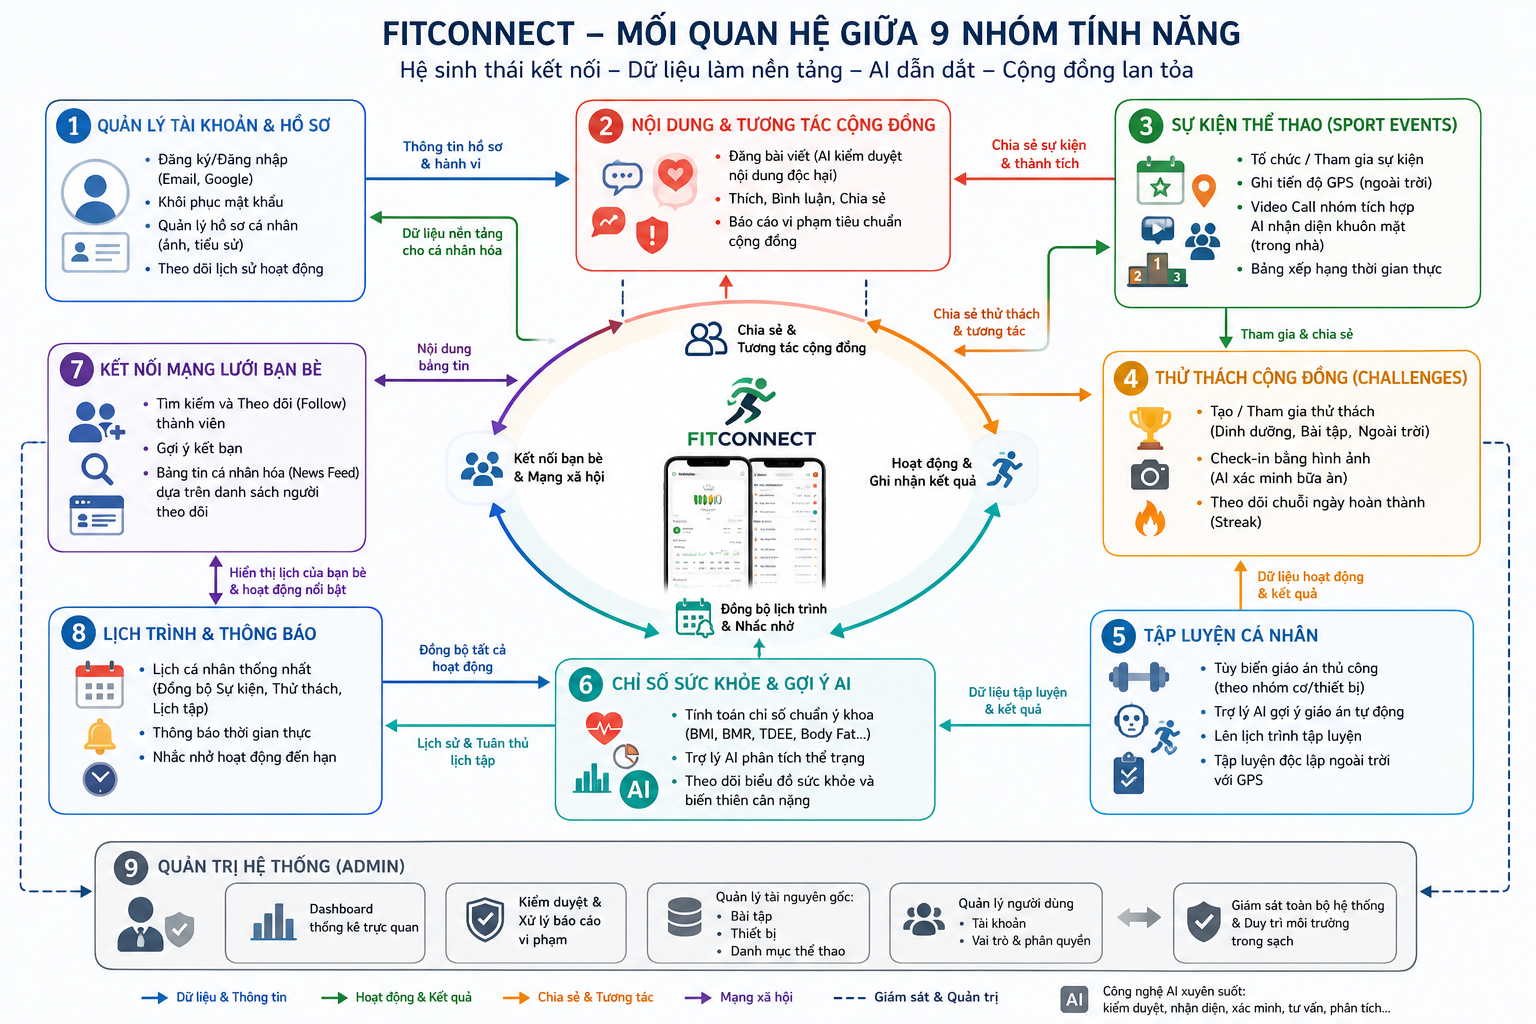
\includegraphics[width=\textwidth]{Images/IMG/Motahethong.png}
\caption{Minh họa khái niệm hệ sinh thái khép kín và mối quan hệ giữa các nhóm tính năng (FitConnect).}
\label{fig:ch1:ecosystem}
\end{figure}

\section{Hiện trạng các nền tảng thể thao -- xã hội và nhu cầu thực tiễn}
\label{sec:intro:platform_status}

Trên bình diện toàn cầu và trong nước, sự giao thoa giữa ``Social'' (mạng xã hội) và ``Fitness'' (thể hình/sức khỏe) đang là xu hướng tất yếu. Các cá nhân tham gia vào hoạt động thể thao thường trải qua ba giai đoạn quá trình tâm lý: \textbf{Khởi đầu (cần hướng dẫn) $\rightarrow$ Duy trì (cần động lực) $\rightarrow$ Tỏa sáng (cần sự công nhận)}\footnote{\href{https://doi.org/10.1186/1479-5868-9-78}{Teixeira et al., IJBNPA, 2012 (động lực \& duy trì hành vi)}}.

\begin{figure}[htbp]
\centering
\setlength{\abovecaptionskip}{14pt}%
\setlength{\belowcaptionskip}{8pt}%
\begin{tikzpicture}[font=\small,
  st/.style={rectangle, draw=black!55, rounded corners=2pt, minimum width=3.6cm, minimum height=1cm, align=center}]
\node[st, fill=gray!12] (s1) at (0,0) {\textbf{Khởi đầu}\\cần hướng dẫn};
\node[st, fill=gray!12] (s2) at (4.8,0) {\textbf{Duy trì}\\cần động lực};
\node[st, fill=gray!12] (s3) at (9.6,0) {\textbf{Tỏa sáng}\\cần sự công nhận};
\draw[->, thick] (s1) -- (s2);
\draw[->, thick] (s2) -- (s3);
\path (current bounding box.south west) ++(0,-0.2) (current bounding box.south east) ++(0,-0.2);
\end{tikzpicture}\par\nobreak\vspace{10pt}\nobreak
\begingroup
\captionsetup{font=footnotesize,labelfont=bf}
\caption{Ba giai đoạn tâm lý thường gặp khi tham gia hoạt động thể thao có hỗ trợ công nghệ.}
\label{fig:ch1:psych-stages}
\endgroup
\end{figure}

Khảo sát thực tiễn cho thấy các ứng dụng hiện hành đang bỏ ngỏ hoặc chưa tối ưu những khoảng trống sau:

\begin{enumerate}
    \item \textbf{Sự kết nối giữa thể dục thể thao ngoài trời (outdoor) và trong nhà (indoor) trong khâu tổ chức sự kiện:} Rất hiếm nền tảng cho phép người dùng chạy bộ ngoài công viên và người dùng đang tập gym tại nhà có thể tham gia chung một ``sự kiện tiến độ cộng đồng'' một cách đồng bộ.

    \item \textbf{Động lực bền bỉ từ thử thách cộng đồng đa dạng:} Các ứng dụng thường chỉ đo lường một loại hình duy nhất. Nhu cầu cần một chuỗi thử thách mạnh mẽ, từ việc kỷ luật \textbf{ăn uống} (có hệ thống AI nhận diện bữa ăn hợp lệ theo thời gian thực), thử thách \textbf{ngoài trời} (đạp xe, chạy bộ) đến lộ trình \textbf{thể dục cá nhân} do AI tư vấn.

    \item \textbf{Cảm giác ``cùng nhau'' từ xa:} Việc tập thể thao ở nhà một mình dễ gây nhàm chán. Nhu cầu kết nối trực tuyến qua luồng video (video call) để tập cùng bạn bè, đồng thời có AI tính toán quy đổi thành điểm số của nhóm là một điểm chạm tương tác chưa được khai thác sâu.

    \item \textbf{Hệ sinh thái thông minh thống nhất:} Ít nền tảng mang lại luồng dữ liệu thông suốt, nơi công cụ tính toán sức khỏe (BMI, TDEE, BMR) chuyển hóa dữ liệu giúp AI chuyên môn gợi ý hệ thống bài tập (workouts) và tự động đồng bộ hóa lên lịch cá nhân (calendar) của người dùng.
\end{enumerate}

Chính bối cảnh này mở ra định hướng thiết kế cốt lõi cho nền tảng FitConnect: \textbf{Lấy tính cộng đồng làm nền tảng, lấy Sự kiện \& Thử thách làm động lực trung tâm, và lấy AI làm công cụ hỗ trợ thông minh.}

\section{Mục tiêu của đề tài}
\label{sec:intro:objectives}

Việc triển khai đề tài hướng tới thỏa mãn các mục tiêu toàn diện ở cả khía cạnh học thuật, công nghệ lẫn ứng dụng thực tiễn:

\begin{enumerate}
    \item \textbf{Mục tiêu sản phẩm:} Xây dựng thành công và đưa vào vận hành hệ thống mạng xã hội thể dục thể thao cộng đồng đa nền tảng (web-based, kiến trúc responsive). Hệ thống phải đảm bảo hoạt động mượt mà, thân thiện với người dùng và xử lý tốt tính liên tục của luồng dữ liệu (news feed, real-time messaging, tracking).

    \item \textbf{Mục tiêu công nghệ \& kỹ thuật:}
    \begin{itemize}
        \item Xây dựng kiến trúc hệ thống hiện đại dựa trên mô hình client--server, áp dụng các tiêu chuẩn thiết kế kiến trúc vi dịch vụ hoặc modular monolithic để mở rộng tính năng dễ dàng.
        \item Ứng dụng trí tuệ nhân tạo (generative AI \& computer vision) một cách sâu rộng vào bài toán thực tiễn: từ việc kiểm tra tính hợp lệ của bài đăng cộng đồng, phân tích hình ảnh nhận diện tiến độ, đến gợi ý lịch trình tập luyện.
        \item Nghiên cứu và hiện thực thành công công nghệ xử lý dữ liệu thời gian thực (real-time GPS tracking, WebSockets cho hệ thống thông báo đa kênh, xử lý đánh giá video stream qua AI)\footnote{\href{https://socket.io/docs/v4/}{Socket.IO docs}; \href{https://datatracker.ietf.org/doc/html/rfc6749}{RFC 6749 (OAuth 2.0)}}.
    \end{itemize}

    \item \textbf{Mục tiêu giá trị xã hội:} Cung cấp một ứng dụng sạch, lành mạnh, tạo ra những cuộc thi/thử thách thể thao mang tính xây dựng, góp phần nâng cao tính kỷ luật, sức khỏe toàn diện cho thanh niên Việt Nam nói riêng và cộng đồng nói chung.
\end{enumerate}

\section{Đối tượng và phạm vi nghiên cứu}
\label{sec:intro:scope}

Để đảm bảo tính khả thi và mức độ hoàn thiện chuyên sâu trong khuôn khổ một đồ án tốt nghiệp, đề tài được giới hạn và phân rã rõ theo các phương diện sau:

\subsection{Đối tượng hướng đến}
\label{subsec:intro:target_audience}

Hệ thống phục vụ đa dạng các tệp người dùng, bao gồm:

\begin{itemize}
    \item \textbf{Người dùng cá nhân:} Những người có nhu cầu chơi thể thao, theo dõi sức khỏe, mong muốn tìm kiếm một lịch trình phù hợp, kết bạn hoặc tham gia các lời mời thử thách.
    \item \textbf{Người khởi xướng sự kiện (event creators/KOLs):} Các hội nhóm thể thao, huấn luyện viên, những nhà hoạt động cộng đồng muốn tổ chức các chiến dịch sức khỏe, phong trào nội bộ hoặc các cuộc thi marathon trực tuyến.
    \item \textbf{Quản trị viên (system admin):} Đội ngũ vận hành hệ thống quản lý dữ liệu master, theo dõi analytics biểu đồ, thực thi kiểm duyệt nội dung và kiểm soát các chỉ số tăng trưởng của nền tảng.
\end{itemize}

\subsection{Phạm vi chức năng}
\label{subsec:intro:functional_scope}

Đồ án tập trung phát triển một hệ thống toàn diện phân rã thành chín nhóm tính năng dành cho người dùng và một phân hệ quản trị (admin), cụ thể:

\subsubsection{Các nhóm tính năng chính}

\begin{enumerate}
    \item \textbf{Cộng đồng:} Xây dựng không gian giao lưu, tương tác mạng xã hội, chia sẻ bài viết, tìm hiểu sự kiện và thử thách. Tích hợp AI tự động kiểm duyệt và nhận diện hình ảnh/nội dung không hợp lệ.

    \item \textbf{Sự kiện thể thao:} Nơi người dùng tạo hoặc tham gia các sự kiện để hoàn thành mục tiêu tập thể. Bao gồm:
    \begin{itemize}
        \item \textbf{Sự kiện ngoài trời:} Hỗ trợ ghi nhận tiến độ bằng GPS tích hợp. Người dùng có thể tham gia sự kiện hoàn thành mục tiêu chung cùng mọi người.
        \item \textbf{Sự kiện trong nhà:} Kết nối thành viên trực tuyến định dạng video call có trợ lực AI nhằm nhận diện và tính toán thời gian vận động thực tế để quy đổi thành tiến độ.
    \end{itemize}

    \item \textbf{Thử thách:} Nền tảng tự rèn luyện cá nhân, nơi người dùng có thể tự tạo hoặc mời bạn bè cùng tham gia. Khác với chức năng sự kiện (tập trung vào mục tiêu tập thể), thử thách đề cao tiến độ bền bỉ mỗi ngày của từng cá nhân. Gồm ba phân loại:
    \begin{itemize}
        \item \textbf{Ăn uống:} Check-in hình ảnh bữa ăn mỗi ngày; hệ thống sử dụng module AI verification đối chiếu hình ảnh để xác thực tính hợp lệ so với yêu cầu đề ra.
        \item \textbf{Ngoài trời:} Ghi lại tiến độ chạy bộ, đạp xe\ldots\ để tiến gần đến mục tiêu cá nhân hằng ngày.
        \item \textbf{Thể dục (gym):} Báo cáo tiến độ hoàn thành các bài tập giúp rèn luyện sức khỏe bản thân.
    \end{itemize}
\end{enumerate}

\subsubsection{Các tính năng bổ trợ quan trọng}

\begin{enumerate}
\setcounter{enumi}{3}
    \item \textbf{Bạn bè:} Quản lý danh sách mạng lưới kết bạn, tăng tính gắn kết trong hệ sinh thái.

    \item \textbf{Tập luyện:} Hệ thống cho phép người dùng tự thiết lập bộ bài tập dựa trên cấu hình tùy chỉnh (thiết bị, nhóm cơ), hoặc nhờ AI cá nhân hóa và gợi ý lộ trình tập. Cung cấp khả năng lưu trữ thành bài tập theo lịch trình dài hạn hoặc các hoạt động ngoài trời độc lập.

    \item \textbf{Công cụ tính toán (calculators):} Bộ công cụ tính các chỉ số sức khỏe sinh học (BMI, BMR, TDEE\ldots), quản lý và hiển thị biểu đồ lịch sử biến động. Dựa vào ngân hàng dữ liệu này, AI insight sẽ tư vấn sức khỏe dựa trên các số đo thực tế và đề xuất phân loại bài tập phù hợp.
    Trong module ước tính tiêu hao năng lượng khi vận động, hệ thống sử dụng công thức quy đổi từ MET sang kcal/phút: $\mathrm{kcal/phút}=\dfrac{MET \times 3.5 \times cân\ nặng\ (kg)}{200}$\footnote{\href{https://pacompendium.com/unite-conversions/}{Compendium of Physical Activities -- Unit Conversions}}. Công thức này dựa trên định nghĩa chuẩn $1\,MET = 3.5\,ml\,O_2/kg/phút$ và quy ước chuyển đổi tiêu hao oxy sang năng lượng, giúp chuẩn hóa cách ước tính giữa các loại hoạt động khác nhau. Nhằm hỗ trợ người dùng phổ thông dễ tra cứu và áp dụng, báo cáo cũng đối chiếu cách diễn giải thực hành từ một tài liệu sức khỏe cộng đồng\footnote{\href{https://howdyhealth.tamu.edu/use-metabolic-equivalents-mets-to-calculate-calories-burned/}{Texas A\&M Howdy Health -- Use METs to Calculate Calories Burned}}.

    \item \textbf{Lịch cá nhân (calendar):} Giao diện lịch biểu hợp nhất, giúp người dùng trực quan hóa lịch trình chéo giữa: thử thách, sự kiện thể thao tham gia và thời khóa biểu các bài tập.

    \item \textbf{Quản lý thông tin cá nhân:} Module authentication, quản lý hồ sơ và các cài đặt tùy biến định danh người dùng.

    \item \textbf{Thông báo:} Kênh notification theo thời gian thực (real-time).
\end{enumerate}

\subsubsection{Phân hệ quản trị (admin panel)}

\begin{enumerate}
\setcounter{enumi}{9}
    \item \textbf{Quản trị hệ thống:} Giao diện dành cho đội ngũ vận hành.
    \begin{itemize}
        \item Cung cấp không gian dashboard trực quan chuyên sâu với các biểu đồ thống kê đa chiều về tình trạng hệ thống.
        \item Công cụ quản lý, trích xuất dữ liệu, kiểm duyệt vi phạm (báo cáo nội dung xấu), ban hành danh mục đối tượng (người dùng, sự kiện, bài viết, đề mục thể thao, tập hợp trang thiết bị thiết yếu, bài tập căn bản và thử thách cộng đồng).
    \end{itemize}
\end{enumerate}

\subsection{Phạm vi kỹ thuật}
\label{subsec:intro:technical_scope}

Kiến trúc hệ thống được xây dựng trên tech-stack hiện đại, tuân thủ các quy tắc design pattern do yêu cầu về tốc độ và chi phí tính toán:

\begin{itemize}
    \item \textbf{Ngôn ngữ và frontend (client-side):} Kiến trúc single page application (SPA) phát triển trên nền tảng ReactJS (sử dụng Vite bundler), tối ưu giao diện component bằng TailwindCSS. Cấu trúc chuyên biệt tách biệt frontend người dùng và frontend quản trị viên\footnote{\href{https://react.dev}{React}; \href{https://vite.dev}{Vite}; \href{https://tailwindcss.com}{Tailwind CSS}}.

    \item \textbf{Backend (API server):} Môi trường Node.js kết hợp TypeScript đảm bảo nguyên tắc type-safe, triển khai qua Express framework theo kiến trúc RESTful kết hợp mô hình lớp controller -- service -- repository\footnote{\href{https://nodejs.org}{Node.js}; \href{https://expressjs.com}{Express}; \href{https://www.typescriptlang.org}{TypeScript}}.

    \item \textbf{Cơ sở dữ liệu (database):} Cấu trúc lõi NoSQL (MongoDB) phục vụ lưu trữ luồng dữ liệu schema-less dạng feed và mạng lưới quan hệ lỏng lẻo của social network\footnote{\href{https://www.mongodb.com/docs/}{MongoDB Documentation}}.

    \item \textbf{Streaming \& công nghệ phụ trợ:} Giao thức WebSockets (Socket.IO) đảm nhận tín hiệu và thông báo thời gian thực; tích hợp API OpenAI cho module đánh giá ngôn ngữ và thị giác. Bảo vệ API có thể áp dụng rate limiting và Helmet\footnote{\href{https://helmetjs.github.io/}{Helmet (HTTP headers, Express)}; \href{https://github.com/express-rate-limit/express-rate-limit}{\texttt{express-rate-limit} (GitHub)}}.
\end{itemize}

\section{Phương pháp nghiên cứu và thực hiện}
\label{sec:intro:methodology}

Quy trình thực hiện đồ án tuân thủ theo chuẩn phát triển phần mềm Agile\footnote{\href{https://agilemanifesto.org}{Agile Manifesto}}, gồm 5 bước: (1)~Nghiên cứu tài liệu về kiến trúc mạng xã hội, thuật toán nhận diện ảnh và prompt engineering; (2)~Khảo sát và đặc tả yêu cầu qua mô hình hóa user personas và use-case; (3)~Thiết kế kiến trúc hệ thống bằng UML (ERD, activity/sequence diagram), phác thảo UI/UX; (4)~Hiện thực theo từng sprint, ánh xạ nghiệp vụ xuống các REST API độc lập; (5)~Kiểm thử toàn diện (unit test, integration test, UAT) đảm bảo độ ổn định và bảo mật.

\section{Bố cục của báo cáo}
\label{sec:intro:structure}

Nội dung cuốn đồ án được tổ chức một cách hệ thống và logic, bao gồm tám chương cụ thể như sau:

\begin{itemize}
    \item \textbf{Chương 1: Giới thiệu đề tài.} Trình bày bối cảnh, lý do chọn đề tài, xác định mục tiêu, đối tượng, phạm vi nghiên cứu và phương pháp thực hiện.

    \item \textbf{Chương 2: Khảo sát hệ thống liên quan.} Đánh giá và phân tích ưu khuyết điểm của các nền tảng mạng xã hội thể thao hiện có trên thị trường, từ đó so sánh và rút ra định hướng thiết kế cốt lõi cho hệ thống FitConnect.

    \item \textbf{Chương 3: Phân tích và đặc tả yêu cầu hệ thống.} Phân tích bài toán thực tế, xác định các tác nhân (actors), lập danh sách các yêu cầu chức năng, phi chức năng và xây dựng biểu đồ use-case bao quát hoạt động.

    \item \textbf{Chương 4: Thiết kế kiến trúc hệ thống.} Cung cấp cái nhìn chuyên sâu về kiến trúc tổng thể, mô hình cơ sở dữ liệu (ERD), thiết kế giao diện (UI/UX) và luồng xử lý dữ liệu qua activity/sequence diagram.

    \item \textbf{Chương 5: Tìm hiểu công nghệ.} Trình bày cơ sở lý thuyết và kỹ thuật áp dụng (Vite/React, Node.js/Express, MongoDB, WebSockets, lý thuyết tích hợp AI và computer vision).

    \item \textbf{Chương 6: Hiện thực hệ thống.} Cụ thể hóa quá trình lập trình thực tế, minh họa cách các phân hệ đi vào hoạt động, những khó khăn thiết kế và giao diện người dùng.

    \item \textbf{Chương 7: Kiểm thử hệ thống.} Trình bày chiến lược kiểm thử, tích hợp các kịch bản test (test cases) nhằm đảm bảo tính đúng đắn, an toàn và hiệu năng thực tế của nền tảng.

    \item \textbf{Chương 8: Tổng kết.} Lập báo cáo kết quả đạt được đối chiếu với mục tiêu đặt ra, tổng kết những khuyết điểm còn tồn đọng và định hướng mở rộng hệ thống trong tương lai.
\end{itemize}
